\documentclass[english]{article}

%% Packages pull in extra commands:
%% http://en.wikibooks.org/wiki/LaTeX/Packages

\usepackage{hyperref}
\usepackage[latin9]{inputenc}
\usepackage[letterpaper]{geometry}
\geometry{verbose,tmargin=1in,bmargin=1in,lmargin=1in,rmargin=1in}
\usepackage{amsmath}
\usepackage{amssymb}
\usepackage{graphicx}
\usepackage{float}
\usepackage{array}
\usepackage{enumerate}
\usepackage{tikz}
\usepackage{bm}

\newcommand\independent{\protect\mathpalette{\protect\independenT}{\perp}}
\def\independenT#1#2{\mathrel{\rlap{$#1#2$}\mkern2mu{#1#2}}}

% New commands serve as shorthand for frequently used command combinations.
\newcommand{\ind}[1]{\mathbf{1}\left(#1\right)}
\newcommand{\bx}{\mathbf{x}}
\newcommand{\E}{\mathbf{E}}

\title{CIS 520, Machine Learning, Fall 2018: Assignment 7}
\author{Shubhankar Patankar}

\begin{document}
\maketitle

{\normalsize \noindent Collaborators: \\ 
\\ \underline{Simran Arora}} \\

\section{Hidden Markov Models}
For the following four probabilities, we want to find $P(X_{1:2} = (sing, TV) | z_{1:2} = (a,b))$ for states $a, b \in \{Happy, \: Sad\}:$
\begin{enumerate}
    \item $(a, \: b) = (Happy,\: Happy)$ \\ \\ 
    	The probability of the first state being Happy state is $P\{Z_1 = Happy\} = (\frac{1}{2})$. Given this first state, the $Pr(Sing, \: Happy) = \frac{5}{10}$. Using the transition probabilities $Pr(Z_{t+1} = Happy | Z_{t} = Happy) = \frac{4}{5}$ and the $Pr(TV | Happy) = \frac{2}{10}$, by the multiplication rule, the total probability of the situation $(a, \; b)$ is $(\frac{1}{2})(\frac{5}{10})(\frac{4}{5})(\frac{2}{10}) = \frac{40}{1000} = 0.04$
    \item $(a, \: b) = (Happy,\: Sad)$ \\ \\
    	The probability of the first state being a Happy state is $P\{Z_1 = Happy\} = (\frac{1}{2})$. Given this first state, the $Pr(Sing, \: Happy) = \frac{5}{10}$. Using the transition probabilities $Pr(Z_{t+1} = Sad | Z_{t} = Happy) = \frac{1}{5})$ and the $Pr(TV | Happy) = \frac{7}{10}$, by the multiplication rule, the total probability of the situation $(a, \; b)$ is $(\frac{1}{2})(\frac{5}{10})(\frac{1}{5})(\frac{7}{10}) = \frac{35}{1000} = 0.035$
    \item $(a, \: b) = (Sad,\: Happy)$ \\ \\
    	The probability of the first state being a Sad state is $P\{Z_1 = Sad\} = (\frac{1}{2})$. Given this first state, the $Pr(Sing, \: Sad) = \frac{1}{10}$. Using the transition probabilities $Pr(Z_{t+1} = Happy | Z_{t} = Sad) = \frac{1}{2})$ and the $Pr(TV | Happy) = \frac{2}{10}$, by the multiplication rule, the total probability of the situation $(a, \; b)$ is $(\frac{1}{2})(\frac{1}{10})(\frac{1}{2})(\frac{2}{10}) = \frac{2}{400} = 0.005$
    \item $(a, \: b) = (Sad,\: Sad)$ \\ \\
    	The probability of the first state being a sad state is $P\{Z_1 = Sad\} = (\frac{1}{2})$. Given this first state, the $Pr(Sing, \: Sad) = \frac{1}{10}$. Using the transition probabilities $Pr(Z_{t+1} = Sad | Z_{t} = Sad) = \frac{1}{2})$ and the $Pr(TV | Sad) = \frac{7}{10}$, by the multiplication rule, the total probability of the situation $(a, \; b)$ is $(\frac{1}{2})(\frac{1}{10})(\frac{1}{2})(\frac{7}{10}) = \frac{7}{400} = 0.0175$
\end{enumerate}
	Based on these probabilities, the most likely hidden state sequence $Z_{1:2} = (Happy, \: Happy)$, with probability $0.04$. Individually, if $(sing, TV)$ are observed then the most likely state for day $2$ is $Sad$ because the $Pr(Sad, Sad) + Pr(Happy, Sad) > Pr(Sad, Happy) + Pr(Happy, Happy)$. The probability of day 2 being Sad is $0.035 + 0.0175 = 0.0525$, while the probability of day 2 being Happy is $0.04 + 0.005 = 0.045$. \newline\newline
	Without any observed actions on the days (i.e. ignoring the fact that (Sing and TV) are observed), from the onset, the most likely hidden state on day $2$ is computed by the total probability formula as follows. $P(Z_2 = Happy) = Pr(Z_2 = Happy | Z_1 = Happy)Pr(Z_1 = Happy) + Pr(Z_2 = Happy | Z_1 = Sad)Pr(Z_1 = Sad) = (\frac{4}{5})(\frac{1}{2}) + (\frac{1}{2})(\frac{1}{2}) = \frac{4}{10} + \frac{1}{4} = 0.65$. Meanwhile  $P(Z_2 = Sad) = Pr(Z_2 = Sad | Z_1 = Happy)Pr(Z_1 = Happy) + Pr(Z_2 = Sad | Z_1 = Sad)Pr(Z_1 = Sad) = (\frac{1}{5})(\frac{1}{2}) + (\frac{1}{2})(\frac{1}{2}) = \frac{1}{10} + \frac{1}{4} = 0.35$. Thus we can see that the individually most likely hidden state on day $2$ is the Happy state.  

\newpage
\section{Missing Data}
\begin{enumerate}
    \item $$Test \;\; Accuracy \;\; Full = 0.9600$$
    \item \textbf{Random NaNs} \\ \\
    Method 1: $Test \;\; Accuracy = 0.9200$ \\
    Method 2: $Test \;\; Accuracy = 0.8667$ 
    \item \textbf{Non-Random NaNs} \\ \\
    Method 1: $Test \;\; Accuracy = 0.9333$ \\
    Method 2: $Test \;\; Accuracy = 0.9467$
    \item Method 1 (mean imputation) is more accurate than Method 2 (indicator variables) for randomly missing data. Method 2 is more accurate for data that is not missing at random. Both methods are less accurate overall than the case when no data is missing. Imputing the mean when the data is not missing at random adds noise to the data making Method 1 less desirable to Method 2, which makes no assumptions about the nature of the missing values. On the other hand, for randomly missing data, adding indicators is less useful than imputing the means because the means of a feature resemble the missing values more than they do when the data is not missing at random. The lack of order in randomly missing data is conducive to mean imputation. Both methods outperform the case where neither Method 1 nor Method 2 is employed, because both methods provide some additional information that is unavailable in the original data. The additional information can only help the ML method being used.
    \end{enumerate}

\newpage
\section{Bayesian Networks}
\begin{enumerate}
    \item $P(x_1, x_2, x_3, x_4, x_5, x_6) = p(x_1)p(x_2)p(x_3 | x_1, x_2)p(x_4| x_2)p(x_6| x_3, x_4)p(x_5| x_3)$
    \item Yes. The joint probability distribution $P'$ in $3.2$ can be represented in the class of joint probability distributions $P$ given by the Bayesian network. In $P'$ we have a subset of $P$ because $P'$ takes $P$ without the dependency of $X_6$ on $X_4$; without the dependency of $X_3$ on $X_1$ or $X_2$; and without the dependency of $X_4$ on $X_2$. Since $P'$ has more independent random variable relationships (more conditional independencies), it is a subset of $P$. Some of the conditional dependencies in $P$ are redundant in the case of $P'$. $P$ is general and is able to represent the given joint probability distribution in $3.2$.
    \item Smaller. Without the edge from $X_3$ to $X_6$ we have $X_6 \independent X_2  | X_4$ instead of $X_6 \independent X_2  | X_4, X_3, X_1$. The resulting network will represent a  narrower class of distributions than the original network because of the fewer dependencies. There are more conditional independencies associated with the resulting network so the resulting network will be smaller than the original network. 
    \item \begin{enumerate}
    \item This is \textbf{FALSE} because there is an active trail for $X_3 \leftarrow X_2 \rightarrow X_4$ where $X_2$ is not observed. In $D-Separation$ we know that variable $X_i$ and $X_j$ are independent if and only if there is no active trail between $X_i$ and $X_j$. Thus we have that $X_3$ and $X_4$ are not independent unless we have observed $X_2$ to remove the active trail. 
    \item This is \textbf{TRUE} because we know by the Local Markov Assumption that a variable $X$ is independent of its non-descendants given its parents. In this case, $X_1$ has no parents and $X_4$ is a non-descendant. Thus, we have that $X_1$ and $X_4$ are independent and by definition of independence, this means that $p(x_1, x_4) = p(x_1)p(x_4)$
    \item This is \textbf{FALSE} for $p(x_1, x_2 | x_6)$. There is an active trail $X_1 \rightarrow X_3 \rightarrow X_6$ and there is an active trail $X_2 \rightarrow X_3 \rightarrow X_6$. We cannot say that $X_1$ and $X_2$ are conditionally independent given $X_6$. 
    % \item This is \textbf{TRUE} for $p(x_1, x_6 | x_3)$. There is no active path from $X_1$ to $X_6$. In the path $X_1 \rightarrow X_3 \rightarrow X_6$, $X_3$ is observed and thus it is not an active path. In D-Separation, we know that variables $X_i$ and $X_j$ are independent if there is no active trail between $X_i$ and $X_j$. Thus, we can conclude that $X_1$ and $X_6$ are independent given $X_3$. By definition of independence, this means that $p(x_1, x_6 | x_3) = p(x_1 | x_3)p(x_6 | x_3)$
    \item This is \textbf{FALSE} for $p(x_1, x_6 | x_3)$. There is an active path from $X_1$ to $X_6$. Since $X_3$ is observed, $X_1$ and $X_2$ are dependent. Since $X_3$ is observed, $X_3$ and $X_4$ have an active trail through $X_2$. Since $X_4$ is not observed, $X_2$ and $X_6$ are dependent. Since both $X_1$ and $X_6$ have active trails from $X_2$ and all consecutive triples in $X_1$ to $X_3$ to $X_2$ to $X_4$ to $X_6$ have active trails, $X_1$ and $X_6$ have an active trail between each other.
    \end{enumerate}
\end{enumerate} 

\newpage
\section{Belief Net Construction}
For this problem, two probabilities are assumed to be equal if they are within $0.05$ of each other. 
\begin{enumerate}
    \item \textbf{Determining Dependencies} \\ \\
    First add A to the belief net. Then add B. Check if B has a trail from A:
    $$P(B \;|\; A) = \frac{1600}{3000} = 0.5333$$
    $$P(B \;|\; \neg A) = \frac{800}{1400} = 0.5714$$
    $$P(B) = \frac{2400}{4400} = 0.5455$$
    $$|P(B \;|\; A) - P(B)| = 0.0122 < 0.05$$
    $$|P(B \;|\; \neg A) - P(B)| = 0.0259 < 0.05$$
    Therefore, B does not depend on A.
    Next, test C.
    $$P(C \;|\; A,B) = \frac{800}{1600} = 0.5$$
    $$P(C \;|\; \neg A, B) = \frac{600}{800} = 0.75$$
    $$P(C \;|\; A, \neg B) = \frac{1200}{1400} = 0.8571$$
    $$P(C \;|\; \neg A, \neg B) = \frac{400}{600} = 0.6667$$
    $$P(C) = \frac{3000}{4400} = 0.6818$$
    $$|P(C \;|\; A,B) - P(C)| = 0.1818 > 0.05$$
    $$|P(C \;|\; \neg A,B) - P(C)| = 0.0682 > 0.05$$
    $$|P(C \;|\; A,\neg B) - P(C)| = 0.1753 > 0.05$$
    $$|P(C \;|\; \neg A,\neg B) - P(C)| = 0.0151 < 0.05$$
    Since $P(C \;|\; A,B) \neq P(C \;|\; \neg A,B) \neq P(C \;|\; A, \neg B) \neq P(C)$, C is linked to the preceding variables.
    Primary test for C's link with A:
    $$P(C \;|\; A) = \frac{2000}{3000} = 0.6667$$
    $$P(C \;|\; \neg A) = \frac{1000}{1400} = 0.7143$$
    $$P(C) = 0.6818$$
    $$|P(C \;|\; A) - P(C)| = 0.0151 < 0.05$$
    $$|P(C \;|\; \neg A) - P(C)| = 0.0325 < 0.05$$
    Therefore, seemingly C does not appear to depend on A. \\
    Primary test for C's link with B:
     $$P(C \;|\; B) = \frac{1400}{2400} = 0.5833$$
    $$P(C \;|\; \neg B) = \frac{1600}{2000} = 0.8$$
    $$P(C) = 0.6818$$
    $$|P(C \;|\; B) - P(C)| = 0.0985 > 0.05$$
    $$|P(C \;|\; \neg B) - P(C)| = 0.1182 > 0.05$$
    Therefore, C depends on B.
    Secondary test for joint dependence of C on B with A.
    $$|P(C \;|\; B, A) - P(C \;|\; B)| = 0.0833 > 0.05$$
    $$|P(C \;|\; B, \neg A) - P(C \;|\; B)| = 0.1667 > 0.05$$
    Since $P(C \;|\; B, A) \neq P(C \;|\; \neg A, B) \neq P(C \;|\; B)$, knowing something about A tells us something about C conditioned on B. Therefore a link is present between A and C. The same inference can be drawn from the inequalities below. 
    $$|P(C \;|\; A, \neg B) - P(C \;|\; \neg B)| = 0.0571 > 0.05$$
    $$|P(C \;|\; \neg A, \neg B) - P(C \;|\; \neg B)| = 0.1333 > 0.05$$
    Next, test D.
    $$P(D \;|\; A,B,C) = \frac{600}{800} = 0.75$$
    $$P(D \;|\; \neg A,B,C) = \frac{200}{600} = 0.3333$$
    $$P(D \;|\; A, \neg B,C) = \frac{400}{1200} = 0.3333$$
    $$P(D \;|\; A,B,\neg C) = \frac{0}{800} = 0$$
    $$P(D \;|\; \neg A,\neg B,C) = \frac{200}{500} = 0.5$$
    $$P(D \;|\; A,\neg B,\neg C) = \frac{0}{200} = 0$$
    $$P(D \;|\; \neg A,B,\neg C) = \frac{0}{200} = 0$$
    $$P(D \;|\; \neg A,\neg B,\neg C) = \frac{0}{200} = 0$$
    $$P(D) = \frac{1400}{4400} = 0.3182$$
        
    $$|P(D \;|\; A,B,C) - P(D)| = 0.4318 > 0.05$$
    $$|P(D \;|\; \neg A,B,C) - P(D)| = 0.0148 < 0.05$$
    $$|P(D \;|\; A,\neg B,C) - P(D)| = 0.0151 < 0.05$$
    $$|P(D \;|\; A,B,\neg C) - P(D)| = 0.3182 > 0.05$$
    $$|P(D \;|\; \neg A,\neg B,C) - P(D)| = 0.1818 > 0.05$$
    $$|P(D \;|\; A,\neg B,\neg C) - P(D)| = 0.3182 > 0.05$$
    $$|P(D \;|\; \neg A,B,\neg C) - P(D)| = 0.3182 > 0.05$$
    $$|P(D \;|\; \neg A,\neg B,\neg C) - P(D)| = 0.3182 > 0.05$$
    
    Since all terms in the differences above are not equal to $P(D)$, D depends on the previously added variables. \\
    Primary test for D's link with A:
    $$P(D \;|\; A) = \frac{1000}{3000} = 0.3333$$
    $$P(D \;|\; \neg A) = \frac{400}{1400} = 0.2857$$
    $$|P(D \;|\; A) - P(D)| = 0.0151 < 0.05$$
    $$|P(D \;|\; \neg A) - P(D)| = 0.0325 < 0.05$$
    Therefore, seemingly D does not appear to depend on A. \\
    
    Primary test for D's link with B:
    $$P(D \;|\; B) = \frac{800}{2400} = 0.3333$$
    $$P(D \;|\; \neg B) = \frac{600}{2000} = 0.3$$
    $$|P(D \;|\; B) - P(D)| = 0.0151 < 0.05$$
    $$|P(D \;|\; \neg B) - P(D)| = 0.0182 < 0.05$$
    Therefore, seemingly D does not appear to depend on B. \\
    
    Primary test for D's link with C:
    $$P(D \;|\; C) = \frac{1400}{3000} = 0.4667$$
    $$P(D \;|\; \neg C) = \frac{0}{1400} = 0.3182$$
    $$|P(D \;|\; C) - P(C)| = 0.1485 > 0.05$$
    $$|P(D \;|\; \neg C) - P(C)| = 0.3182 > 0.05$$
    Therefore, D depends on C. \\
    
    Secondary test for joint dependence of D on C with A and/or B.
    $$P(D \;|\; A, C) = \frac{1000}{2000} = 0.5$$
    $$P(D \;|\; B, C) = \frac{800}{1400} = 0.5714$$
    $$|P(D \;|\; A, C) - P(D \;|\; C)| =  0.0333 < 0.05$$
    $$|P(D \;|\; B, C) - P(D \;|\; C)| =  0.1047 > 0.05$$
    Therefore, knowing B tells us more about D conditioned on C, implying that B and D are linked.
    $$P(D \;|\; \neg A, C) = \frac{400}{1000} = 0.4$$
    $$|P(D \;|\; \neg A, C) - P(D \;|\; C)| =  0.0667 > 0.05$$
    $$|P(C \;|\; B, \neg A) - P(C \;|\; B)| = 0.1667 > 0.05$$
    Therefore, knowing A tells us more about D conditioned on C, implying that A and D are also linked.
    
    \begin{figure}[H]
    \centering
    \includegraphics[scale = 0.5]{belief_net}
    \caption{Constructed Belief Net}
    \label{fig:belief_net}
    \end{figure}
    
    \underline{Conditional Probability Tables} \\ \\
    The table below outlines the probabilities of C given values of A and B.
    \begin{figure}[H]
    \centering
    \includegraphics[scale = 0.5]{T1}
    % \caption{Constructed Belief Net}
    \label{fig:T1}
    \end{figure}
    
    The table below outlines the probabilities of C given values of A, B and C.
    \begin{figure}[H]
    \centering
    \includegraphics[scale = 0.5]{T2}
    % \caption{Constructed Belief Net}
    \label{fig:T2}
    \end{figure}
    
    $P(A) = 0.6818$, $P(B) = 0.5455$, $P(C) = 0.6818$
    
\end{enumerate}

\newpage
\section{EM}
\begin{enumerate}
    \item \textbf{Model Parameters} \\
    $$p(D_i,C_i,A_i,B_i) = p(D_i|C_i,A_i,B_i) \times p(C_i|A_i,B_i) \times p(A_i|B_i) \times p(B_i)$$
    However, based on the belief net structure,
    $$p(D_i,C_i,A_i,B_i) = p(D_i|C_i) \times p(C_i|A_i,B_i) \times p(A_i) \times p(B_i)$$
    Therefore the model parameters $\bm{\theta$} are: \\
    $p(D_i|C_i)$, $p(D_i|\neg C_i)$, $p(C_i|A_i,B_i)$, $p(C_i|\neg A_i,B_i)$, $p(C_i|A_i,\neg B_i)$, $p(C_i|\neg A_i,\neg B_i)$, $p(A_i)$ and $p(B_i)$.
    
    \[ p(D_i \;|\; C_i = 1) = \begin{cases} 
    p_1 & D_i = 1\\
    1-p_1 & D_i = 0 \\
    \end{cases}
    \]
    $$\therefore p(D_i \;|\; C_i = 1) = {p_1}^{D_i}(1-p_1)^{1-D_i}$$
    
    \[ p(D_i \;|\; C_i = 0) = \begin{cases} 
    p_2 & D_i = 1\\
    1-p_2 & D_i = 0 \\
    \end{cases}
    \]
    $$\therefore p(D_i \;|\; C_i = 0) = {p_2}^{D_i}(1-p_2)^{1-D_i}$$
    
    \[ p(C_i \;|\; A_i = 1, B_i = 1) = \begin{cases} 
    p_3 & C_i = 1\\
    1-p_3 & C_i = 0 \\
    \end{cases}
    \]
    $$\therefore p(C_i \;|\; A_i = 1, B_i = 1) = {p_3}^{C_i}(1-p_3)^{1-C_i}$$
    
    \[ p(C_i \;|\; A_i = 0, B_i = 1) = \begin{cases} 
    p_4 & C_i = 1\\
    1-p_4 & C_i = 0 \\
    \end{cases}
    \]
    $$\therefore p(C_i \;|\; A_i = 0, B_i = 1) = {p_4}^{C_i}(1-p_4)^{1-C_i}$$
    
    \[ p(C \;|\; A_i = 1, B_i = 0) = \begin{cases} 
    p_5 & C_i = 1\\
    1-p_5 & C_i = 0 \\
    \end{cases}
    \]
    $$\therefore p(C_i \;|\; A _i = 1, B_i = 0) = {p_5}^{C_i}(1-p_5)^{1-C_i}$$
    
    \[ p(C \;|\; A_i = 0, B_i = 0) = \begin{cases} 
    p_6 & C_i = 1\\
    1-p_6 & C_i = 0 \\
    \end{cases}
    \]
    $$\therefore p(C_i \;|\; A_i = 0, B_i = 0) = {p_6}^{C_i}(1-p_6)^{1-C_i}$$
    
    \[ p(A_i) = \begin{cases} 
    p_7 & A_i = 1\\
    1-p_7 & A_i = 0 \\
    \end{cases}
    \]
    $$\therefore p(A_i) = {p_7}^{A_i}(1-p_7)^{1-A_i}$$
    
    \[ p(B_i) = \begin{cases} 
    p_8 & B_i = 1\\
    1-p_8 & B_i = 0 \\
    \end{cases}
    \]
    $$\therefore p(B_i) = {p_8}^{B_i}(1-p_8)^{1-B_i}$$
    
    \item \textbf{E-Step} \\ \\
    For the given belief net, the observed states are $\mathbf{x_i} = \{A_i, B_i, D_i\}$. \\
    $$C_i = z \in \{0,1\}$$
    The full joint distribution including the hidden state $C_i$ can be written as follows:
    $$p(D_i,C_i,A_i,B_i) = \big[{p_1}^{D_i}(1-p_1)^{1-D_i}\big]^{C_i} \times \big[{p_2}^{D_i}(1-p_2)^{1-D_i}\big]^{1-C_i} \times$$
    $$\big[{p_3}^{C_i}(1-p_3)^{1-C_i}\big]^{A_iB_i} \times \big[{p_4}^{C_i}(1-p_4)^{1-C_i}\big]^{(1-A_i)B_i} \times \big[{p_5}^{C_i}(1-p_5)^{1-C_i}\big]^{(1-B_i)A_i} \times$$
    $$\big[{p_6}^{C_i}(1-p_6)^{1-C_i}\big]^{(1-A_i)(1-B_i)} \times \big[{p_7}^{A_i}(1-p_7)^{1-A_i}\big] \times \big[{p_8}^{B_i}(1-p_8)^{1-B_i}\big]$$
    \\ 
    $$\therefore p(C_i = z \;|\; \mathbf{x_i}, \bm{\theta}^{t-1}) = \frac{p(\mathbf{x_i} \;|\;  C_i = z) p(C_i = z)}{p(\mathbf{x_i})} = \frac{p(\mathbf{x_i},C_i = z)}{\sum_{C_i} p(\mathbf{x_i}, C_i = z)}$$
    Equivalently, this can be written as:
    $$p(C_i = z\;|\; \mathbf{x_i}, \theta^{t-1}) = \frac{p(\mathbf{x_i}, C_i = z \;|\; \theta^{t-1})}{p(\mathbf{x_i}, C_i = 1 \;|\; \theta^{t-1}) + p(\mathbf{x_i}, C_i = 0 \;|\; \theta^{t-1})} = \frac{p(\mathbf{x_i}, C_i = z \;|\; \theta^{t-1})}{\sum_{C_i} p(\mathbf{x_i}, C_i = z)}$$
    Or as:
    $$p(C_i = z\;|\; \mathbf{x_i}, \theta^{t-1}) = \frac{p(D_i,C_i = z,A_i,B_i)}{\sum_{C_i} p(D_i,C_i = z,A_i,B_i)}$$

    \item \textbf{M-Step} \\ \\
    $$\bm{\theta}^t = arg max_{\bm{\theta}} \; q(\bm{\theta},\bm{\theta^{t-1}})$$
    $$ q(\bm{\theta},\bm{\theta}^{t-1}) = \sum_{i}\sum_{C_i}p(C_i \;|\; \mathbf{x_i}, \bm{\theta}^{t-1}) \times ln \; p(\mathbf{x_i},C_i \;|\; \bm{\theta})$$
    $$ = \sum_{i} \bigg[ \big[p(C_i = 1 \;|\; \mathbf{x_i}, \bm{\theta}^{t-1}) \; ln \; p(\mathbf{x_i},C_i = 1 \;|\; \bm{\theta})\big] + \big[ p(C_i = 0 \;|\; \mathbf{x_i}, \bm{\theta}^{t-1}) \; ln \; p(\mathbf{x_i},C_i = 0 \;|\; \bm{\theta}) \big] \bigg]$$
    
    $$\because p(D_i,C_i,A_i,B_i) = p(D_i|C_i) \times p(C_i|A_i,B_i) \times p(A_i) \times p(B_i)$$
    $$ \implies ln \; p(\mathbf{x_i},C_i = z \;|\; \bm{\theta}) = ln \; P(D_i | C_i = z) + ln \; P(C_i = z| A_i, B_i)  + ln \; P(A_i) + ln \; P(B_i)$$
    Each of the $ln$ terms in $q(\bm{\theta},\bm{\theta}^{t-1})$ can be substituted for with the above expression, appropriately replacing $z$. 
    
    % $$ = \sum_{i} \bigg[ \frac{p(\mathbf{x_i}, C_i = 1 \;|\; \bm{\theta}^{t-1}) \big[ln \; p(\mathbf{x_i},C_i = 1 \;|\; \bm{\theta})\big]}{p(\mathbf{x_i}, C_i = 1 \;|\; \bm{\theta}^{t-1}) + p(\mathbf{x_i}, C_i = 0 \;|\; \bm{\theta}^{t-1})}  + \frac{p(\mathbf{x_i}, C_i = 0 \;|\; \bm{\theta}^{t-1})\big[ln \; p(\mathbf{x_i},C_i = 0 \;|\;\bm{\theta})\big]}{p(\mathbf{x_i}, C_i = 1 \;|\; \bm{\theta}^{t-1}) + p(\mathbf{x_i}, C_i = 0 \;|\; \bm{\theta}^{t-1})}\bigg] $$
    % $$ = \sum_{i} \bigg[ \frac{p(\mathbf{x_i}, C_i = 1 \;|\; \theta^{t-1}) \big[ln \; p(\mathbf{x_i},C_i = 1 \;|\; \bm{\theta})\big]}{\sum_{C_i} p(\mathbf{x_i}, C_i)}  + \frac{p(\mathbf{x_i}, C_i = 0 \;|\; \theta^{t-1})\big[ln \; p(\mathbf{x_i},C_i = 0 \;|\; \bm{\theta})\big]}{\sum_{C_i} p(\mathbf{x_i}, C_i)}\bigg] $$
    
    \item \textbf{(C, D) or (C and D) Missing} \\ \\
    Since C is missing for the first half of the samples, the same updates as above can be used for $i = 1:(1/2)n$, where $n$ is the total number of samples. 
    $$i = 1:(1/2)n$$
    $$C_i = z \in \{0,1\}$$
    $$\mathbf{x_i} = \{A_i, B_i, D_i\}$$ 
    \underline{E-Step}:
    $$p(C_i = z\;|\; \mathbf{x_i}, \theta^{t-1}) = \frac{p(\mathbf{x_i}, C_i = z \;|\; \theta^{t-1})}{p(\mathbf{x_i}, C_i = 1 \;|\; \theta^{t-1}) + p(\mathbf{x_i}, C_i = 0 \;|\; \theta^{t-1})} = \frac{p(\mathbf{x_i}, C_i = z \;|\; \theta^{t-1})}{\sum_{C_i} p(\mathbf{x_i}, C_i = z)}$$
    \underline{M-Step}:
    $$\bm{\theta}^t = arg max_{\bm{\theta}} \; q(\bm{\theta},\bm{\theta^{t-1}})$$
    $$ q(\bm{\theta},\bm{\theta}^{t-1}) = \sum_{i}\sum_{C_i}p(C_i = z\;|\; \mathbf{x_i}, \bm{\theta}^{t-1}) \times ln \; p(\mathbf{x_i},C_i = z\;|\; \bm{\theta})$$
    $$q(\bm{\theta},\bm{\theta}^{t-1}) = \sum_{i} \bigg[ \big[p(C_i = 1 \;|\; \mathbf{x_i}, \bm{\theta}^{t-1}) \; ln \; p(\mathbf{x_i},C_i = 1 \;|\; \bm{\theta})\big] + \big[ p(C_i = 0 \;|\; \mathbf{x_i}, \bm{\theta}^{t-1}) \; ln \; p(\mathbf{x_i},C_i = 0 \;|\; \bm{\theta}) \big] \bigg]$$
  
    $$ \because ln \; p(\mathbf{x_i},C_i = z \;|\; \bm{\theta}) = ln \; P(D_i | C_i = z) + ln \; P(C_i = z| A_i, B_i)  + ln \; P(A_i) + ln \; P(B_i)$$
    Each of the $ln$ terms in $q(\bm{\theta},\bm{\theta}^{t-1})$ can be substituted for with the above expression, appropriately replacing $z$.
    
    D is missing for the next quarter of the samples. 
    $$i = (1/2)n:(3/4)n$$
    $$D_i = w \in \{0,1\}$$
    $$\mathbf{x_i} = \{A_i, B_i, C_i\}$$ 
    \underline{E-Step}:
    $$p(D_i = z\;|\; \mathbf{x_i}, \theta^{t-1}) = \frac{p(\mathbf{x_i}, D_i = w \;|\; \theta^{t-1})}{p(\mathbf{x_i}, D_i = 1 \;|\; \theta^{t-1}) + p(\mathbf{x_i}, D_i = 0 \;|\; \theta^{t-1})}$$
    \underline{M-Step}:
    $$\bm{\theta}^t = arg max_{\bm{\theta}} \; q(\bm{\theta},\bm{\theta^{t-1}})$$
    $$ q(\bm{\theta},\bm{\theta}^{t-1}) = \sum_{i}\sum_{D_i}p(D_i = w\;|\; \mathbf{x_i}, \bm{\theta}^{t-1}) \times ln \; p(\mathbf{x_i},D_i = w\;|\; \bm{\theta})$$
    $$q(\bm{\theta},\bm{\theta}^{t-1}) = \sum_{i} \bigg[ \big[p(D_i = 1 \;|\; \mathbf{x_i}, \bm{\theta}^{t-1}) \; ln \; p(\mathbf{x_i},D_i = 1 \;|\; \bm{\theta})\big] + \big[ p(D_i = 0 \;|\; \mathbf{x_i}, \bm{\theta}^{t-1}) \; ln \; p(\mathbf{x_i},D_i = 0 \;|\; \bm{\theta}) \big] \bigg]$$
    
    $$ \because ln \; p(\mathbf{x_i},D_i = w \;|\; \bm{\theta}) = ln \; P(D_i = w | C_i) + ln \; P(C_i | A_i, B_i)  + ln \; P(A_i) + ln \; P(B_i)$$
    Each of the $ln$ terms in $q(\bm{\theta},\bm{\theta}^{t-1})$ can be substituted for with the above expression, appropriately replacing $w$.
    
    Both C and D are missing for the final quarter of the samples.
    
    $$i = (3/4)n:n$$
    $$\mathbf{x_i} = \{A_i, B_i\}$$ 
    $$C_i = z \in \{0,1\}$$
    $$D_i = w \in \{0,1\}$$
    \underline{E-Step}:
    $$p(C_i = z, D_i = w\;|\; \mathbf{x_i}, \theta^{t-1}) = \frac{p(\mathbf{x_i}, C_i = z D_i = w \;|\; \theta^{t-1})}{\sum_{C_i} \sum_{D_i} p(\mathbf{x_i}, C_i, D_i)}$$
    \underline{M-Step}:
    $$\bm{\theta}^t = arg max_{\bm{\theta}} \; q(\bm{\theta},\bm{\theta^{t-1}})$$
    $$ q(\bm{\theta},\bm{\theta}^{t-1}) = \sum_{i}\sum_{C_i}\sum_{D_i}p(C_i = z, D_i = w \;|\; \mathbf{x_i}, \bm{\theta}^{t-1}) \times ln \; p(\mathbf{x_i},C_i = z,D_i = w \;|\; \bm{\theta})$$
      
     $$ \because ln \; p(\mathbf{x_i},C_i = z, D_i = w \;|\; \bm{\theta}) = ln \; P(D_i = w | C_i = z) + ln \; P(C_i = z | A_i, B_i)  + ln \; P(A_i) + ln \; P(B_i)$$
    Each of the $ln$ terms in $q(\bm{\theta},\bm{\theta}^{t-1})$ can be substituted for with the above expression, appropriately replacing $z$ and $w$ for the possible values of $C_i$ and $D_i$, respectively.
      
\end{enumerate}

\end{document}